\documentclass{beamer}
\usetheme{Metropolis}  % Use the Metropolis theme
\usepackage{tikz}      % For precise positioning
\usepackage{booktabs}


\title{LUS Image Classification of Covid-19 and Pneumonia}
\author{
    \textbf{Abhijith C }\\ % Your name
    242CS003 \\ % Your roll number
    Under the guidance of \textbf{Dr. Jeny Rajan} \\ % Your guide's name
}
\date{\today}

\begin{document}

\maketitle

\section{Introduction}
\begin{frame}{LUS Images}
        Lung ultrasound (LUS) images provide key diagnostic information by capturing different artifacts and structures in the lungs. Key elements in LUS images include:
\begin{itemize}
        \item \textbf{Pleural Line} – The bright, horizontal line at the top of the image, representing the lung’s surface.
        \item \textbf{A-Lines} – Repetitive horizontal artifacts indicating normal aerated lungs.
        \item \textbf{B-Lines} – Vertical, hyperechoic (bright) lines extending to the bottom, associated with lung pathologies like pneumonia and pulmonary edema.
        %\item \textbf{Consolidations} – Hypoechoic (dark) regions indicating areas of lung tissue affected by infection or inflammation.
        %\item \textbf{Pleural Effusion} – Fluid accumulation appearing as an anechoic (black) area beneath the lung.
    \end{itemize}
    
\end{frame}

\begin{frame}{LUS Images}
    \begin{columns}
        \column{0.5\textwidth}
        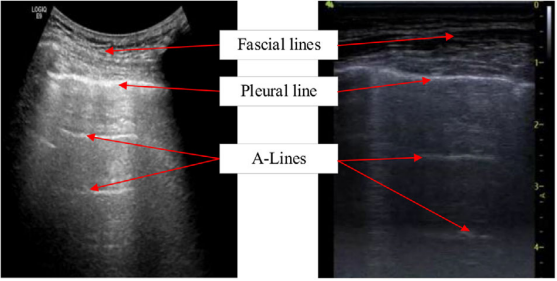
\includegraphics[width=\linewidth]{img/a-lines.png}
        
        \column{0.5\textwidth}
        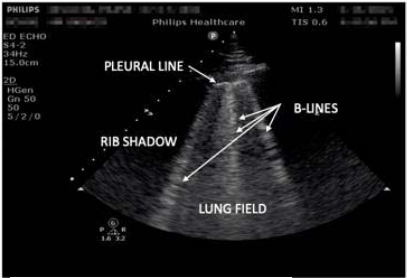
\includegraphics[width=\linewidth]{img/b-lines.png}
    \end{columns}
    \begin{tikzpicture}[remember picture, overlay]
        \node[anchor=south] at (current page.south) {\tiny \textbf{Image Sources: \cite{a-lines}, \cite{b-lines}}};
    \end{tikzpicture}
\end{frame}

\begin{frame}{LUS Differences: COVID-19 vs. Pneumonia}
    \centering
    \begin{tabular}{lll}
        \hline
        \textbf{Feature} & \textbf{COVID-19} & \textbf{Pneumonia} \\
        \hline
        \textbf{B-Lines} & Scattered, widespread & Localized in one area \\
        \hline
        \textbf{Pleural Line} & Thick and uneven & Mostly normal \\
        \hline
        %\textbf{Consolidations} & Less common & More frequent \\
        %\hline
        %\textbf{Pleural Effusion} & Rare & Common \\
        %\hline
        \textbf{Lung Involvement} & Both lungs (bilateral) & One lung (unilateral) \\
        \hline
    \end{tabular}
    
    %\vspace{0.5cm}
    %\centering
    %\includegraphics[width=0.6\textwidth]{example-image}  % Replace with actual LUS image
    
\end{frame}

\section{Dataset}

\begin{frame}{Dataset Overview}
\begin{table}[]
        \centering
        \begin{tabular}{lc}
            \toprule
            \textbf{Label} & \textbf{Count} \\
            \midrule
            COVID-19 & 524 \\
            Pneumonia & 463 \\
            \bottomrule
        \end{tabular}
	\vspace{0.5cm}
        \caption{Dataset Label Distribution}
    \end{table}
\end{frame}

\begin{frame}{Data Loading and Preprocessing}

    \textbf{Data Loading Process:}
    \begin{itemize}
        \item Resize images to uniform dimensions (\(224 \times 224\)).
        \item Convert labels into numerical format (COVID = 0, Pneumonia = 1).
    \end{itemize}

    \textbf{Data Splitting:}
    \begin{itemize}
        \item Train (80\%) + Validation (10\%) + Test (10\%) split.
    \end{itemize}
\end{frame}

\begin{frame}{Data Augmentation Steps}
    \begin{itemize}
        \item \textbf{Geometric Transformations:}
        \begin{itemize}
            \item Rotation: Randomly rotates images by up to \( \pm20^\circ \).
            \item Width Shift: Shifts images horizontally by \( \pm10\% \).
            \item Height Shift: Shifts images vertically by \( \pm10\% \).
            \item Shear: Applies shearing transformation up to \( 0.2 \) radians.
            \item Zoom: Random zooming in/out up to \( \pm20\% \).
            \item Horizontal Flip: Randomly flips images left-right.
        \end{itemize}
        \item \textbf{Fill Mode:} Uses \texttt{nearest} pixel values to fill missing areas.
    \end{itemize}
\end{frame}

\section{Experiments Performed}

\begin{frame}{ResNet50}
    \textbf{Model Architecture:}
    \begin{itemize}
        \item \textbf{Base Model:} Pretrained ResNet50 model with weights trained on ImageNet
        \item \textbf{Custom Layers:}
        \begin{itemize}
            \item Flatten Layer
            \item Fully Connected Layer (512 units, ReLU activation)
            \item Output Layer (1 unit, Sigmoid activation)
        \end{itemize}
        \item \textbf{Loss Function:} Binary Cross-Entropy
        \item \textbf{Optimizer:} Adam (Learning Rate = 0.0001)
    \end{itemize}
\end{frame}

\begin{frame}{ResNet50}
	\centering
     	\includegraphics[width=1\linewidth]{img/resnet\_acc.png}
    	\newline
    	\textbf{Figure:} Accuracy Curve
\end{frame}

\begin{frame}{ResNet50}
	\centering
     	\includegraphics[width=1\linewidth]{img/resnet\_loss.png}
    	\newline
    	\textbf{Figure:} Loss Curve
\end{frame}

\begin{frame}{ResNet50}
	\centering
     	\includegraphics[width=0.8\linewidth]{img/resnet\_confusion.png}
    	\newline
    	\textbf{Figure:} Confusion Matrix
\end{frame}

\begin{frame}{ResNet50}
	\centering
     	\includegraphics[width=1\linewidth]{img/resnet\_test.png}
	\includegraphics[width=1\linewidth]{img/resnet\_report.png}
\end{frame}

\begin{frame}{VGG16}
    \textbf{Model Architecture:}
    \begin{itemize}
        \item \textbf{Base Model:} Pretrained VGG16 model with weights trained on ImageNet
        \item \textbf{Custom Layers:}
        \begin{itemize}
            \item Flatten Layer
            \item Fully Connected Layer (512 units, ReLU activation)
            \item Output Layer (1 unit, Sigmoid activation)
        \end{itemize}
        \item \textbf{Loss Function:} Binary Cross-Entropy
        \item \textbf{Optimizer:} Adam (Learning Rate = 0.0001)
    \end{itemize}
\end{frame}

\begin{frame}{VGG16}
	\centering
     	\includegraphics[width=1\linewidth]{img/vgg\_acc.png}
    	\newline
    	\textbf{Figure:} Accuracy Curve
\end{frame}

\begin{frame}{VGG16}
	\centering
     	\includegraphics[width=1\linewidth]{img/vgg\_loss.png}
    	\newline
    	\textbf{Figure:} Loss Curve
\end{frame}

\begin{frame}{VGG16}
	\centering
     	\includegraphics[width=0.8\linewidth]{img/vgg\_confusion.png}
    	\newline
    	\textbf{Figure:} Confusion Matrix
\end{frame}

\begin{frame}{VGG16}
	\centering
     	\includegraphics[width=1\linewidth]{img/vgg\_test.png}
	\includegraphics[width=1\linewidth]{img/vgg\_report.png}
\end{frame}

\begin{frame}{K-Fold Cross-Validation for ResNet50}
    \textbf{Key Steps:}
    \begin{itemize}
        \item \textbf{Splitting Data:} The dataset is divided into 5 folds.
        \item \textbf{Training \& Validation:} Each fold is used once as validation while the remaining 4 folds are used for training.
        \item \textbf{Performance Evaluation:} Validation accuracy and loss are computed for each fold.
        \item \textbf{Final Model Training:} After 5 iterations, a final model is trained on the full dataset.
        \item \textbf{Test Set Evaluation:} The final model is evaluated on the test set.
    \end{itemize}
\end{frame}

\begin{frame}{K-Fold Cross-Validation for ResNet50}
    \begin{table}[]
        \centering
        \begin{tabular}{cccc}
            \toprule
            \textbf{Fold} & \textbf{Validation Accuracy} & \textbf{Validation Loss}  \\
            \midrule
            Fold 1  & 0.9430  & 0.6063   \\
            Fold 2  & 0.9937  & 0.0074   \\
            Fold 3  & 0.9937  & 0.0267   \\
            Fold 4  & 0.9494  & 1.8617   \\
            Fold 5  & 0.8280  & 40.4298 \\
            \midrule
        \end{tabular}
    \end{table}
	\includegraphics[width=1\linewidth]{img/kfold\_avg.png}
\end{frame}

\begin{frame}{K-Fold Cross-Validation for ResNet50}
	\centering
     	\includegraphics[width=0.8\linewidth]{img/kfold\_confusion.png}
    	\newline
    	\textbf{Figure:} Confusion Matrix
\end{frame}

\begin{frame}{K-Fold Cross-Validation for ResNet50}
	\centering
     	\includegraphics[width=1\linewidth]{img/kfold\_test.png}
	\includegraphics[width=1\linewidth]{img/kfold\_report.png}
\end{frame}

\begin{frame}{ResNet50 with Imbalanced Dataset}
\begin{itemize}
        \item \textbf{Original Class Distribution:} 
        \begin{itemize}
            \item Class 0 (Covid): 524 samples
            \item Class 1 (Pneumonia): 463 samples
        \end{itemize}
        \item \textbf{Imbalanced Class Distribution:} 
        \begin{itemize}
            \item Class 0 (Covid): 524 samples
            \item Class 1 (Pneumonia): 46 samples
        \end{itemize}
    \end{itemize}
\end{frame}

\begin{frame}{ResNet50 with Imbalanced Dataset}
	\centering
     	\includegraphics[width=1\linewidth]{img/imb\_acc.png}
    	\newline
    	\textbf{Figure:} Accuracy Curve
\end{frame}

\begin{frame}{ResNet50 with Imbalanced Dataset}
	\centering
     	\includegraphics[width=1\linewidth]{img/imb\_loss.png}
    	\newline
    	\textbf{Figure:} Loss Curve
\end{frame}

\begin{frame}{ResNet50 with Imbalanced Dataset}
	\centering
     	\includegraphics[width=0.8\linewidth]{img/imb\_confusion.png}
    	\newline
    	\textbf{Figure:} Confusion Matrix
\end{frame}

\begin{frame}{ResNet50 with Imbalanced Dataset}
	\centering
     	\includegraphics[width=1\linewidth]{img/imb\_test.png}
	\includegraphics[width=1\linewidth]{img/imb\_report.png}
\end{frame}

\begin{frame}{Introduction to Vision Transformers (ViTs)}
    \begin{itemize}
        \item Originally designed for \textbf{Natural Language Processing (NLP)}, used in models like \textbf{GPT} and \textbf{BERT}.
        \item \textbf{First applied to computer vision} in 2020 for \textbf{image classification and segmentation} by Dosovitskiy et al. \cite{vit}.
        \item The \textbf{core idea}:
        \begin{itemize}
            \item Instead of convolutional filters, \textbf{images are divided into patches}.
            \item Each patch is treated as a \textbf{token}, similar to words in NLP.
            \item A standard \textbf{Transformer encoder} is used to process these tokens.
        \end{itemize}
	\item Great potential in Ultrasound Image Analysis \cite{vit-us}.
    \end{itemize}
\end{frame}

\begin{frame}{ViT Architecture}
	\centering
    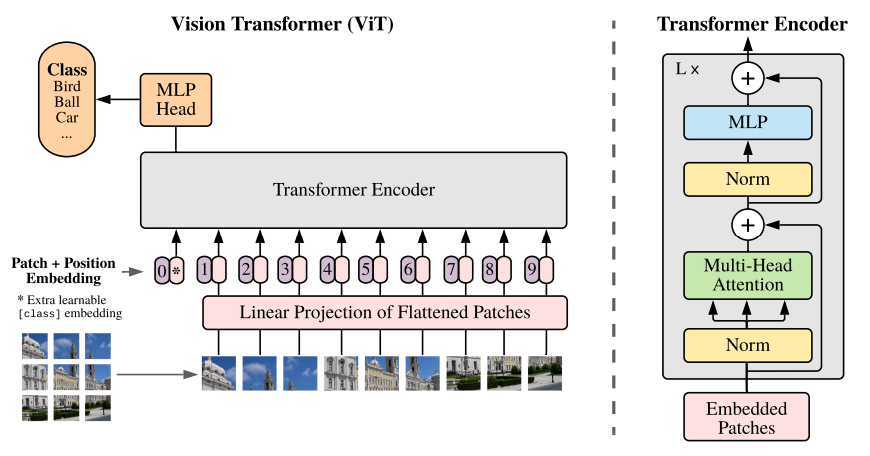
\includegraphics[width=\textwidth]{img/vit_arch.png}
    \newline
\newline
    	\textbf{Figure:} Model Overview of Vision Transformers
    \begin{tikzpicture}[remember picture, overlay]
        \node[anchor=south] at (current page.south) {\tiny \textbf{Image Source: \cite{vit}}};
    \end{tikzpicture}
\end{frame}

\begin{frame}
    \frametitle{Introduction to Swin Transformer}

    \begin{itemize}
        \item Swin Transformer was proposed by Microsoft Research in 2021 \cite{swin}.
\item The \textbf{core idea}:
        \begin{itemize}
            \item Uses a \textbf{shifted window attention mechanism} instead of global self-attention.
            \item Reduces computational complexity compared to ViT.
	\end{itemize}
            \item Captures Fine Details with Local \& Global Features.
            \item Scales well and processes high resolution images faster.
            \item Used in COVID-19 Pneumonia Assessment in Lung Ultrasound Images \cite{swin-lus}.
    \end{itemize}

\end{frame}

\begin{frame}{Swin Tiny Transformer}
\begin{itemize}
    \item \textbf{Base Model:} Swin Tiny Transformer pretrained on ImageNet-1K \\
    \item \textbf{Input Size:} \(224 \times 224 \times 3\) \\
    \item\textbf{Frozen Layers:} All except classification head \\
    \item \textbf{New Classification Head:}
    \begin{itemize}
        \item Linear (num\_features → 256)
        \item ReLU Activation
        \item Dropout (0.5)
        \item Linear (256 → 2 classes)
    \end{itemize}
        \item \textbf{Loss Function:} CrossEntropyLoss
        \item \textbf{Optimizer:} Adam (lr=$1 \times 10^{-4}$, weight decay=$1 \times 10^{-5}$)
        \item \textbf{Scheduler:} StepLR (Step size = 5, Gamma = 0.5)
    \end{itemize}
\end{frame}

\begin{frame}{Swin Tiny Transformer}
	\centering
     	\includegraphics[width=1\linewidth]{img/swin\_acc.png}
    	\newline
    	\textbf{Figure:} Accuracy Curve
\end{frame}

\begin{frame}{Swin Tiny Transformer}
	\centering
     	\includegraphics[width=1\linewidth]{img/swin\_loss.png}
    	\newline
    	\textbf{Figure:} Loss Curve
\end{frame}

\begin{frame}{Swin Tiny Transformer}
	\centering
     	\includegraphics[width=0.6\linewidth]{img/swin\_confusion.png}
    	\includegraphics[width=0.4\linewidth]{img/swin\_test.png}
\end{frame}


\section{Conclusion}
\begin{frame}{Summary}

    \textbf{Performance Metrics for Different Models}  
    \bigskip
    
    \begin{table}[]
        \centering
\resizebox{\textwidth}{!}{
        \begin{tabular}{lcccc}
            \toprule
            \textbf{Model} & \textbf{Train Accuracy} & \textbf{Test Accuracy} & \textbf{Train Loss} & \textbf{Test Loss} \\
            \midrule
            ResNet50 & 99.69 & 100 & 0.0413 & 0.003 \\
	  VGG16  & 97.59 & 100 & 0.1192 & 0.033 \\
	ResNet50 K-Fold  & 99.60 & 94.95 & 0.0123 & 6.3086 \\
            ResNet50 Imbalanced  & 97.79 & 100 & 0.2008  & 0.0057\\
	Swin Transformer & 96.60 & 98.48 & 0.1477 & 0.0783\\
            \bottomrule
        \end{tabular}}
    \end{table}

\end{frame}

\begin{frame}{References}
    \footnotesize
    \begin{thebibliography}{99}
        \bibitem{a-lines} Xing, W., et al. "Automatic detection of A‐line in lung ultrasound using deep learning." Medical Physics 50.1 (2023): 330-343.
        \bibitem{b-lines} Baloescu, C., et al. "Automated lung ultrasound B-line assessment using deep learning." IEEE T-UFFC 67.11 (2020): 2312-2320.
        \bibitem{vit} Dosovitskiy, A., et al. "An image is worth 16x16 words: Transformers for image recognition at scale." arXiv:2010.11929 (2020).
    \end{thebibliography}

\end{frame}

\begin{frame}{References}
    \footnotesize
    \begin{thebibliography}{99}
        \bibitem{swin} Liu, Z., et al. "Swin Transformer: Hierarchical ViT using shifted windows." ICCV (2021).
        \bibitem{vit-us} Vafaeezadeh, M., Behnam, H., \& Gifani, P. "Ultrasound image analysis with vision transformers." Diagnostics 14.5 (2024): 542.
        \bibitem{swin-lus} Fiorentino, M. C., et al. "ViT approaches for COVID-19 pneumonia assessment in lung ultrasound." IEEE MetroXRAINE (2024).
    \end{thebibliography}
\end{frame}

\begin{frame}{}
    \centering
    \vspace{1cm}
    {\LARGE \textbf{Thank You!}} \\

\end{frame}

\end{document}
